\documentclass[a4paper, 11pt]{report}
\usepackage[utf8]{inputenc}
\usepackage[frenchb]{babel}
\usepackage{color}
\usepackage[final]{pdfpages} 
\usepackage{verbatim}

\def\blurb{%
  Université Bordeaux 1 \\
  Master 1 - Informatique \\[1em]
  Mémoire - Projet de Programmation}
\def\clap#1{\hbox to 0pt{\hss #1\hss}}%
\def\ligne#1{%
  \hbox to \hsize{%
    \vbox{\centering #1}}}%
\def\haut#1#2#3{%
  \hbox to \hsize{%
    \rlap{\vtop{\raggedright #1}}%
    \hss
    \clap{\vtop{\centering #2}}%
    \hss
    \llap{\vtop{\raggedleft #3}}}}%
\def\bas#1#2#3{%
  \hbox to \hsize{%
    \rlap{\vbox{\raggedright #1}}%
    \hss
    \clap{\vbox{\centering #2}}%
    \hss
    \llap{\vbox{\raggedleft #3}}}}%
\begin{document}
\thispagestyle{empty}\vbox to .9\vsize{%
  \vss
  \vbox to 1\vsize{%
    \haut{}{\blurb}{}
    \vfill
    \ligne{\Large Création d'IA pour Rasende Roboter}
    \vspace{5mm}
    \ligne{Olivier Braïk
	\\Alexandre Delesse
	\\Gaëtan Lussagnet
	\\Alexandre Mourany
	\\Dimitri Ranc
\\{\today}}
    \vfill
    \ligne{%
      \begin{tabular}{l}
         \\Chargé de TD :  Emmanuel Fleury
      \end{tabular}}
    \vspace{5mm}
    \ligne{%
      \begin{tabular}{l}
	Clients :\\
        Tom Bouvier \\
        Simon Boyé\\
        Jérôme Kirman \\
        Noémie-Fleur Sandillon-Rezer \\
      \end{tabular}
      }
    }%
  \vss
  }

\newpage
\section*{Résumé}
Nous devons proposer aux clients une implémentation du jeu Rasende Roboter sur Mac et Linux. Le programme doit comprendre une partie en solo comprenant les règles basiques du jeu. Les clients ont souhaité ajouter une fonctionnalité qui permet de résoudre le jeu et la possibilité de jouer en réseau.
Ce document présente notre projet, les différents choix de l'architecture ainsi que des parties délicates du code comme la partie en réseau ou l'algorithme de résolution implémenté.

\tableofcontents

\chapter*{Introduction}
\addcontentsline{toc}{chapter}{Introduction}

	Nous devons proposer aux clients une implémentation du jeu Rasende Roboter sur Mac et Linux. Le programme doit comprendre une partie en solo comprenant les règles basiques du jeu. Les clients ont souhaité ajouter une fonctionnalité qui permet de résoudre le jeu et la possibilité de jouer en réseau.

	Rasende Roboter est un jeu de société allemand créé par Alex Randolph et illustré par Franz Vohwinkel, édité en 1999 par Hans im Glück / Tilsit. Le jeu est composé d'un plateau, de tuiles représentant chacune une des cases du plateau, et de pions appelés « robots ». La partie est décomposée en tours de jeu, un tour consistant à déplacer les robots sur un plateau afin d'en amener un sur l'une des cases du plateau. Les robots se déplacent en ligne droite et avancent toujours jusqu'au premier mur qu'ils rencontrent. On peut aussi bien y jouer seul qu'à un grand nombre de participants.
	
	Ce projet s'inscrit dans le cadre de l'UE projet de programmation du second semestre de la première année de Master Informatique. Il est réalisé par une équipe de cinq étudiants du Master spécialité Génie Logiciel, trois étudiants (Olivier Braïk, Gaëtan Lussagnet et Dimitri Ranc) sont en option Programmation multi-coeur et GPU, les deux autres (Alexandre Delesse et Alexandre Mourany) sont en option Administration réseaux. Le projet s'étale sur la totalité du semestre.

\newpage
\null
\newpage

\chapter{Le Projet}

\section{Règles du jeu}
Le jeu est composé d'un plateau formé grâce à 4 quarts de plateau à 2 faces ce qui permet d'obtenir 96 configurations différentes. Le plateau est un quadrillage de 16 par 16 cases dont certaines sont des cases objectif. 

À chaque tour, le ou les joueur(s) reçoivent l'objectif à atteindre. Le but est alors d'amener le robot de la couleur correspondante sur la case objectif dont le symbole est identique à celui de l'objectif. Si l'objectif est multicolore, il faut alors amener n'importe quel robot sur la case multicolore du plateau.

Les joueurs jouent simultanément, chacun réfléchissant sur le moyen d'amener le robot en utilisant les règles de déplacement. Lorsque l'un d'entre eux pense avoir trouvé une solution, il annonce en combien de mouvements il compte atteindre l'objectif puis il active le compte à rebours de 120 secondes. Les autres joueurs ont jusqu'à la fin du compte à rebours pour proposer de meilleures solutions, utilisant moins de mouvements.
Après l'écoulement du temps, le joueur qui a la solution comptant le moins de mouvement montre sa solution et remporte la tuile. S'il échoue dans sa démonstration, le joueur qui proposait le nombre de mouvements immédiatement supérieur montre sa solution, etc. jusqu'à ce qu'une solution soit valide.

\section{Analyse de l'existant}
Le projet consistant à implémenter un jeu de société, nous avons commencé par en étudier les règles. Nous avons donc étudié le jeu original Rasende Roboter. Nous avons ensuite recherché s'il existait une version libre d'un projet similaire au notre. Nous avons fini par trouver plusieurs implémentations différentes (tant par le langage choisi que par la modification des règles originales).
Nous avons notamment trouvé le code développé par une équipe de l'INSA de Rouen qui nous a permis de nous faire une idée générale de ce que nous avions à coder.

\section{Manuel de l'application}
\begin{figure}[!h]
	\centering
   	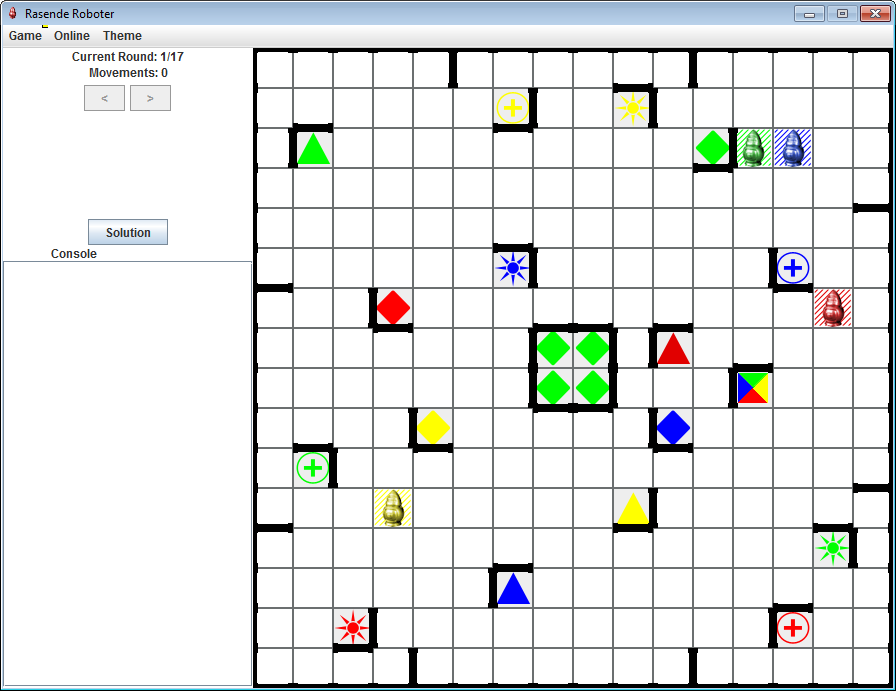
\includegraphics[scale=0.5]{img/interfacegraphique.png}
	\caption{Interface graphique de notre Rasende Roboter}
\end{figure}
Le jeu possède trois composantes importantes : la barre de menu, le panneau de contrôle et le plateau de jeu.

\subsection{Barre de menu}
Le menu "Game" permet de lancer une nouvelle partie en cliquant sur "New Game". Un nouveau plateau de jeu est alors généré avec un nouvel objectif et le compteur de tour est réinitialisé.
En cliquant sur "Help", les règles et le fonctionnement du jeu vous seront rappelés.
Cliquer sur "License" affichera les crédits du jeu, c'est-à-dire les développeurs du jeu, ainsi que la licence utilisée pour le créer.
Pour quitter le jeu il faut cliquer sur le bouton "Quit".
 
Le menu "Online" permet de se mesurer à d'autres joueurs en rejoignant un serveur déjà créé, ou en en créant un soi-même.
Pour rejoindre un serveur, cliquez sur "Join server". Il vous sera alors demandé un nom d'utilisateur ainsi que l'IP du serveur à rejoindre.
 
Pour créer son propre serveur et pouvoir accueillir d'autres joueurs dans votre partie, cliquez sur "Start Server". Seul un nom d'utilisateur vous sera demandé.

Le menu "Theme" vous permettra de choisir entre deux thèmes graphiques : le thème par défaut et le thème Pokemon. D'autres thèmes peuvent facilement être rajoutés si besoin.

\subsection{Panneau de contrôle}
Le panneau de contrôle permet de suivre la progression du jeu et d'effectuer des actions.
\subsubsection{En partie locale}
"Current Round" indique le tour qui est joué.
"Movements" indique le nombre de déplacements qui ont été fait avec les robots pendant le tour actuel.
Le chevron "\textless" permet d'annuler le dernier mouvement effectué et le chevron "\textgreater" permet de rétablir un mouvement qui a été annulé.
Le bouton "Solution" lance un solveur qui calcule le chemin le plus rapide pour arriver sur l'objectif et affiche les déplacements nécessaires dans la console. Il est ensuite affiché dans la console.
\subsubsection{En partie en ligne}
Si la partie en cours est en ligne, les informations disponibles dans le panneau de contrôle ne sont pas exactement les mêmes.
Pour commencer, afin d'éviter la triche, le bouton de solution disparait de la colonne. En revanche, la liste des joueurs connectés et le nombre de point apparaît. Il est aussi possible de proposer son estimation du nombre de coups que l'on prévoit de faire. Le premier joueur qui valide son estimation lance un compteur pendant lequel tout le monde peut proposer son estimation. Une fois que le compteur se termine, les joueurs sont classés selon leur estimation et celui qui a la plus petite prend la main pour montrer le chemin qu'il a trouvé. S'il n'y arrive pas il peut abandonner le tour en cliquant sur "Forfeit" et laisse alors la main au joueur suivant et ainsi de suite ...

\subsection{Le plateau de jeu et déplacement des robots}
\begin{figure}[!h]
   	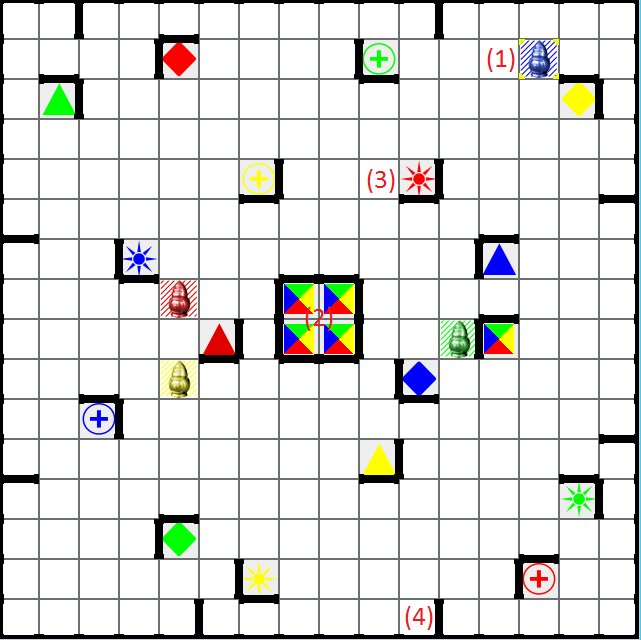
\includegraphics[scale=0.5]{img/plateaudejeu.png}
   	\centering
	\caption{Capture du plateau de jeu pendant un partie}
	Le plateau est un quadrillage contenant les 4 pions, l'objectif, les cases cibles avec leurs murs.
	\begin{enumerate}
		\item Un des quatre pions du jeu. Les cases de départ des pions sont marquées par des rayures de la couleur du robot. Le robot sélectionné est encadré en jaune.
		\item L'objectif à atteindre par les robots.
		\item Une case cible.
		\item Les murs sont représentés par des traits noirs épais.
	\end{enumerate}
\end{figure}

Les robots se déplacent de manière rectiligne jusqu'à rencontrer un obstacle (mur ou autre robot). En partie locale, on peut bouger les robots quand on veut, en revanche en partie en ligne on peut bouger les robots seulement si on a la main.
Il faut d'abord sélectionner un robot. Soit en cliquant dessus soit en utilisant le clavier avec les touches :
\begin{itemize}
	\item R ou 1 pour le robot rouge
	\item V ou 2 pour le robot vert
	\item B ou 3 pour le robot bleu
	\item Y ou 4 pour le robot jaune
\end{itemize}
Ensuite utilisé les flèches directionnelles ou la souris pour déplacer le robot sélectionné dans l'une des quatre directions possibles.



\subsection{Conseils}
En premier lieu, vous apprendrez clairement beaucoup plus de choses en jouant plutôt qu'en lisant cette rubrique qui sera forcément très courte. 
N'oubliez pas que vous pouvez utiliser tous les robots. 
Vérifiez rapidement s'il n'existe pas un chemin direct entre le robot et son objectif (une solution en 6 ou 7 coups). 
Si ce n'est pas le cas, regardez quelles sont les possibilités pour arriver sur la bonne case et quels robots vous pouvez placer en obstacle pour y arriver.
Vous vous êtes trompés en déplaçant un robot ? Utilisez les boutons "<" et ">" pour revenir en arrière ou inversement.
Lors d'une partie en ligne, n'oubliez pas que vous pouvez faire des annonces supérieures à celles déjà faites, le joueur a pu se tromper.
Les solutions en plus de 15 coups sont rares, mais ça arrive. Ce sont évidemment des solutions qui demandent une grande concentration pour être trouvée. Si personne ne trouve de solution (chaque problème à une solution), n'hésitez pas à passer le tour. 
Évitez d'enchaîner les parties, c'est un jeu qui fatigue vite.


\newpage
\null
\newpage

\chapter{Cahier des charges}
\section{Scénario}
Le scénario a été construit grâce au site Mockflow, il a plusieurs fois évolué en fonction des souhaits des clients et des différentes améliorations proposées au fur et à mesure de la programmation.
Voici la maquette de la fenêtre en partie locale :
\begin{figure}[h!]
	\centering
   	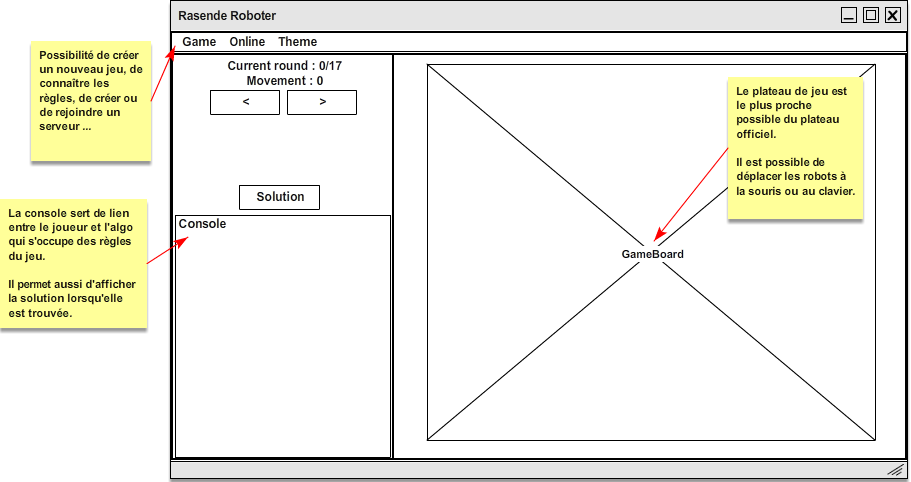
\includegraphics[scale=0.43]{img/local.png}
\end{figure}

L'interface se veut simple et épurée. Le joueur peut déplacer les robots sur le plateau soit à la souris soit avec le clavier pour aller plus vite. Le nombre de mouvement est automatiquement mis à jours jusqu'à ce qu'il atteigne la case objectif.
Si la partie se joue en ligne, de nouveaux éléments s'ajoutent à l'écran, comme la possibilité de proposer un nombre de mouvement ou la liste des joueurs connecté.
\newpage
\section{Besoins fonctionnels}
	\subsection{Jouer en local}
	La fenêtre de jeu en local est divisée en deux :
	\begin{itemize}
	\item A droite, le plateau de jeu.
	\item A gauche, une colonne qui contient :
		\begin{itemize}
		\item Les informations sur le jeu (numéro du tour, nombre de déplacements).
		\item Deux boutons permettant de revenir en arrière ou l'inverse pendant le jeu.
		\item Un bouton permettant de trouver la solution au tour.
		\item Une "console" qui affiche ce que doit faire le joueur à tout moment.
		\end{itemize}
	\end{itemize}

	Le menu de la fenêtre permet de commencer une nouvelle partie (avec un nouveau plateau construit aléatoirement en respectant les plateaux officiels), de quitter le jeu, d'afficher l'aide, de rejoindre ou de créer un serveur et de changer le thème du jeu.

	Spécificités de cet écran :
	\begin{itemize}
	\item Le premier couple de couleur de robot/emplacement à atteindre est défini (un nouveau couple sera redéfini à chaque nouveau tour de jeu).
	\item Déplacement à la souris ou au clavier pour résoudre la partie.
	\item Lorsque le joueur atteint l'objectif le tour est terminé, on choisit alors une nouvelle case objectif.
	\item Une fois les 17 tours terminés, la partie recommence.
	\end{itemize}

	\subsection{Jouer en ligne}
	
	Une partie en ligne débute en créant ou en rejoignant un serveur. Dans les deux cas, on se crée un profil rapide (en saisissant un nom de joueur). Le serveur synchronise tous les clients pour qu'ils aient le même plateau.

La fenêtre est similaire à celle du jeu en local. Cependant, le bouton solution est remplacé par : 
	\begin{itemize}
	\item[-] Un champ servant à proposer sa solution (le nombre de déplacement que l'on prévoit).
	\item Un encart avec la liste des joueurs et leur proposition respective.
	\item Un bouton pour déclarer forfait pendant un tour.
	\end{itemize}

	Spécificités de cet écran :
	\begin{itemize}
	\item Le joueur ne peut pas déplacer les robots, il doit trouver une solution dans sa tête.
	\item Une fois qu'un des joueurs a proposé sa solution, un compteur démarre. Pendant le décompte, chaque joueur peut proposer une proposition (meilleure ou non que la première). A la fin du temps, les joueurs sont classés en fonction de leur proposition. Celui qui a proposé le moins de mouvement prend la main.
	\item Le joueur qui a la main déplace les robots pour atteindre l'objectif. Il a autant de déplacements qu'il a proposé pour y arriver.
	\item Si le joueur ne retrouve pas la solution qu'il avait proposée il déclare forfait pour le tour et c'est le suivant dans le classement qui prend la main et ainsi de suite.
	\item Si personne ne trouve la solution, le tour est fini, on passe au suivant.
	\end{itemize}

	C'est le serveur qui s'occupe du bon fonctionnement de la partie, les clients ne récupèrent qu'une copie de la partie.

\section{Besoins non-fonctionnels}
\subsection{Jouabilité}
Le jeu doit être jouable, il est donc nécessaire d'avoir :
	\begin{itemize}
		\item une interface ergonomique et simple.
		\item des commandes intuitives, avec par exemple la possibilité d'utiliser les flèches pour le déplacement des robots et l'initiale de la couleur du robot pour en sélectionner un.
		\item un temps de réponse correct.
 	\end{itemize}

Il est également nécessaire pour garder un intérêt dans le jeu de tout faire pour éviter les possibilités de triche. Il faut notamment vérifier pendant les parties en réseau qu'il n'y a pas  de possibilité de tricher lorsqu'il y a un temps limite.

\subsection{Systèmes d'exploitation}
Le jeu doit être portable sur Linux et Mac. Pour cela, nous avons décidé de programmer le jeu en Java, plus précisément en Java 7 (il tourne donc aussi sous windows).

\subsection{Réutilisation}
Le choix d'une licence libre permettra au projet de continuer dans le temps et d'être repris. La mise en place d'une documentation (du type Javadoc) est aussi utile pour permettre au code d'être éventuellement modifié dans le futur.
Le code doit permettre une évolution rapide et facile en utilisant des Interfaces, en utilisant des noms de méthodes simples à comprendre, en permettant une lecture claire du code.

\section{Priorités}
	\begin{enumerate}
		\item Partie Solo.
		\item Algorithme trouvant la meilleure solution possible.
		\item Partie en réseau.
		\item En option : possibilité de construire son propre plateau de jeu.
		\item En option: nouvel algorithme plus "humain" permettant de faire des parties face à l'ordinateur en solo.
	\end{enumerate}

\section{Tableau des risques}
\begin{figure}[h!]
	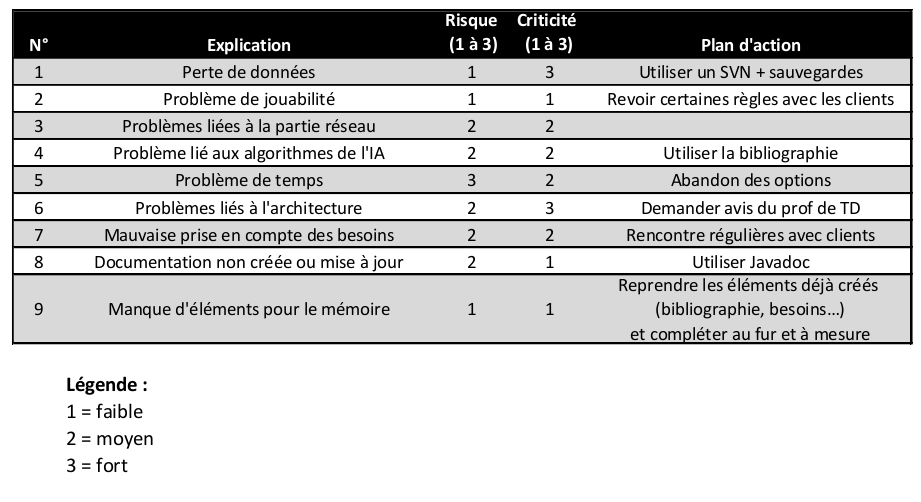
\includegraphics[scale=0.5]{img/risques.png}
\end{figure}

\chapter{Architecture}

	\section{Diagramme de classes}
	\subsection{Diagramme de Packages}
		\begin{figure}[h!]
	   	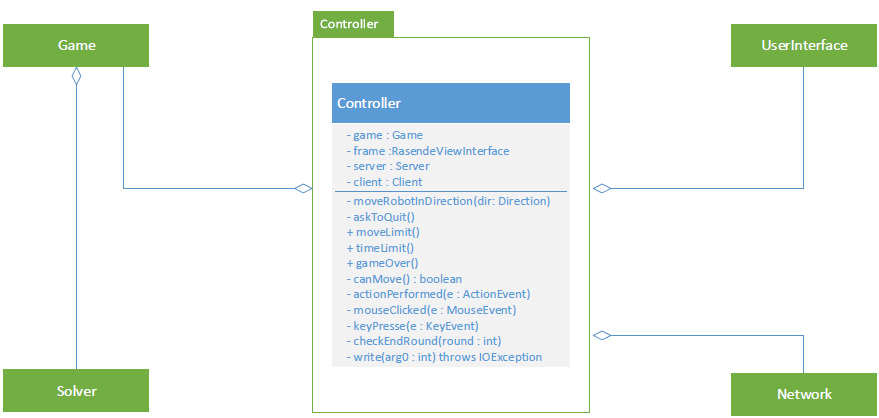
\includegraphics[scale=0.6]{img/packages.png}
		\end{figure}
\newpage
	\subsection{Package Game}
		\begin{figure}[h!]
	   	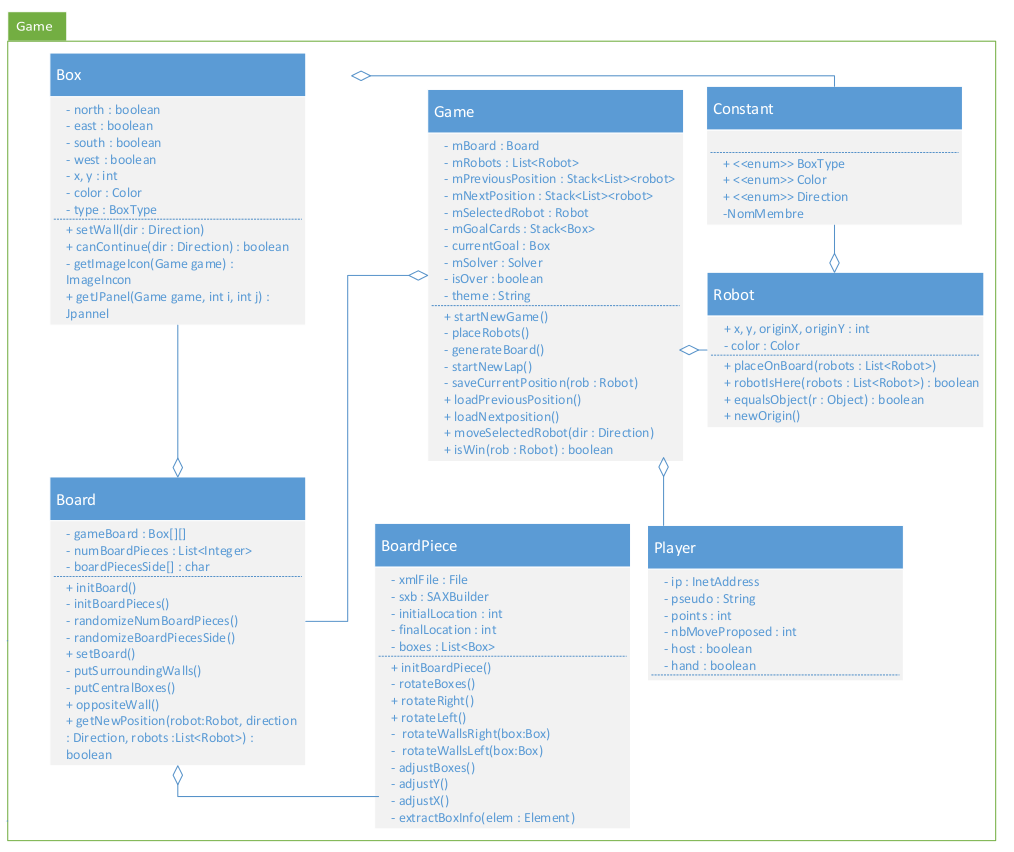
\includegraphics[scale=0.6]{img/game.png}
		\end{figure}
\newpage
	\subsection{Package Network}
		\begin{figure}[h!]
	   	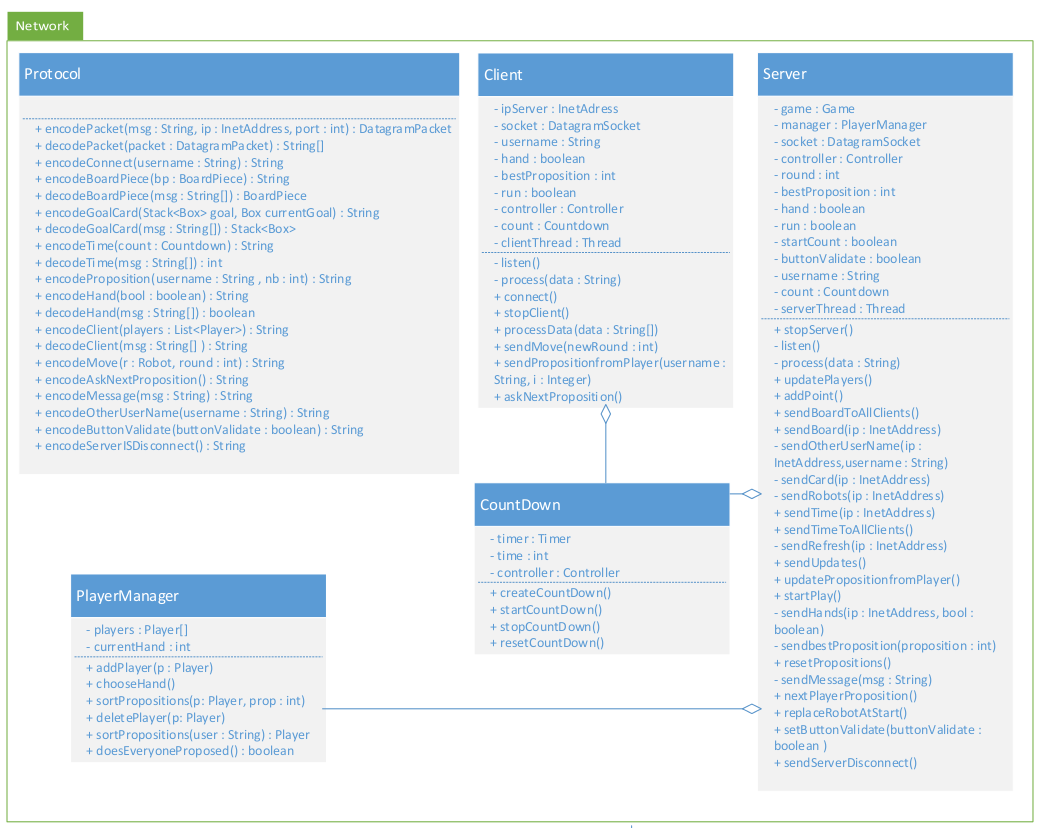
\includegraphics[scale=0.6]{img/network.png}
		\end{figure}
\newpage
	\subsection{Package UserInterface}
		\begin{figure}[h!]
	   	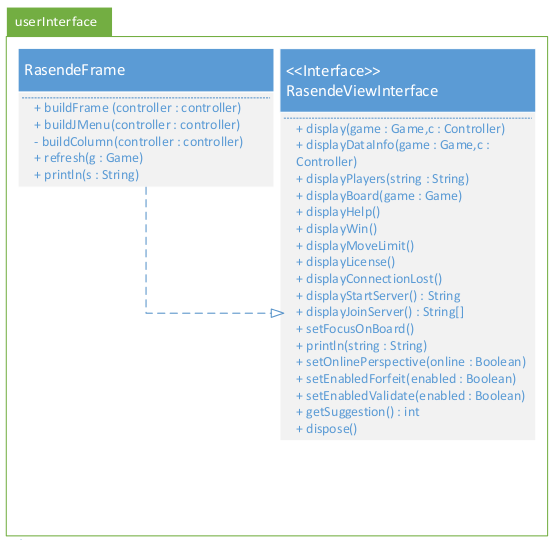
\includegraphics[scale=0.7]{img/userinterface.png}
		\end{figure}
\newpage
	\subsection{Package Solver}
		\begin{figure}[h!]
	   	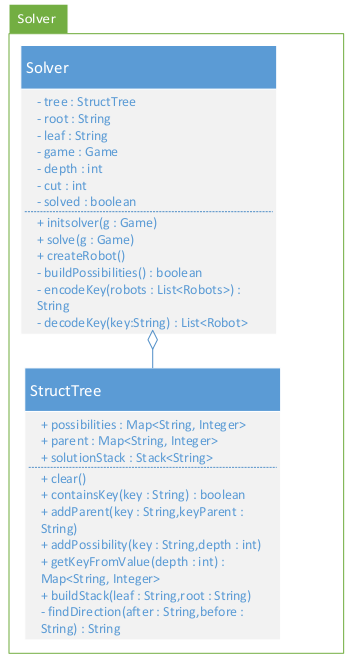
\includegraphics[scale=0.7]{img/solver.png}
		\end{figure}
\newpage
		
	\section{Explications détaillés}
	
	\subsection{MVC}
	
	Nous avons choisi d'utiliser l'architecture Modèle-Vue-Contrôleur pour notre projet de programmation. Notre projet s'organise en plusieurs packages qui représentent les différentes composantes de l'architecture MVC.\\
	
\begin{enumerate}

\item[-]Le package Game correspond à notre modèle. Il contient tous les éléments qui constituent le jeu, comme par exemple les robots ou encore le plateau. 
\item[-]Le package Network contient le code relatif au réseau.
\item[-]Le package Solver contient le code relatif à l'algorithme de résolution de la partie.
\item[-]Le package UserInterface contient la classe qui nous servira à générer une interface graphique. 
\item[-]Dans le package Controller, nous trouvons la classe Controller qui nous servira à faire le lien entre le modèle et la vue. 
\item[-]Le package Main contient la classe Main qui servira au lancement de notre logiciel.
\item[-]Le package Test contiendra les différentes classes où sont effectués les test. Ce package n'a pas d'influence sur notre architecture.

\end{enumerate}

	Le package Game contient les classes Board et BoardPiece qui servent à instancier le plateau de jeu grâce à des fichiers xml. La création des plateaux de jeu est expliquée dans une autre partie de ce rapport. 
	
	La classe Box contient les informations relatives à une case du plateau. C'est à dire si elle contient un symbole objectif, ou encore si elle contient un mur. 
	
	La classe Constant répertorie toutes le constantes que nous utilisons, comme par exemple les couleurs des robots, ou bien les directions possibles pour le déplacement des robots.
	
	 La classe Player contient les informations relatives à un joueur. Cette classe est utilisée dans la partie réseau, elle nous permet d'assigner une adresse ip, ou encore un pseudo à un joueur. 
	 
	 La classe Robot sert à instancier les pions du jeu. 
	 
	 Enfin la classe Game regroupe tous les éléments présentés ci-dessus, elle représente notre modèle.
	 
	 


	Voici un schéma pour montrer comment s'articule notre architecture MVC :
	
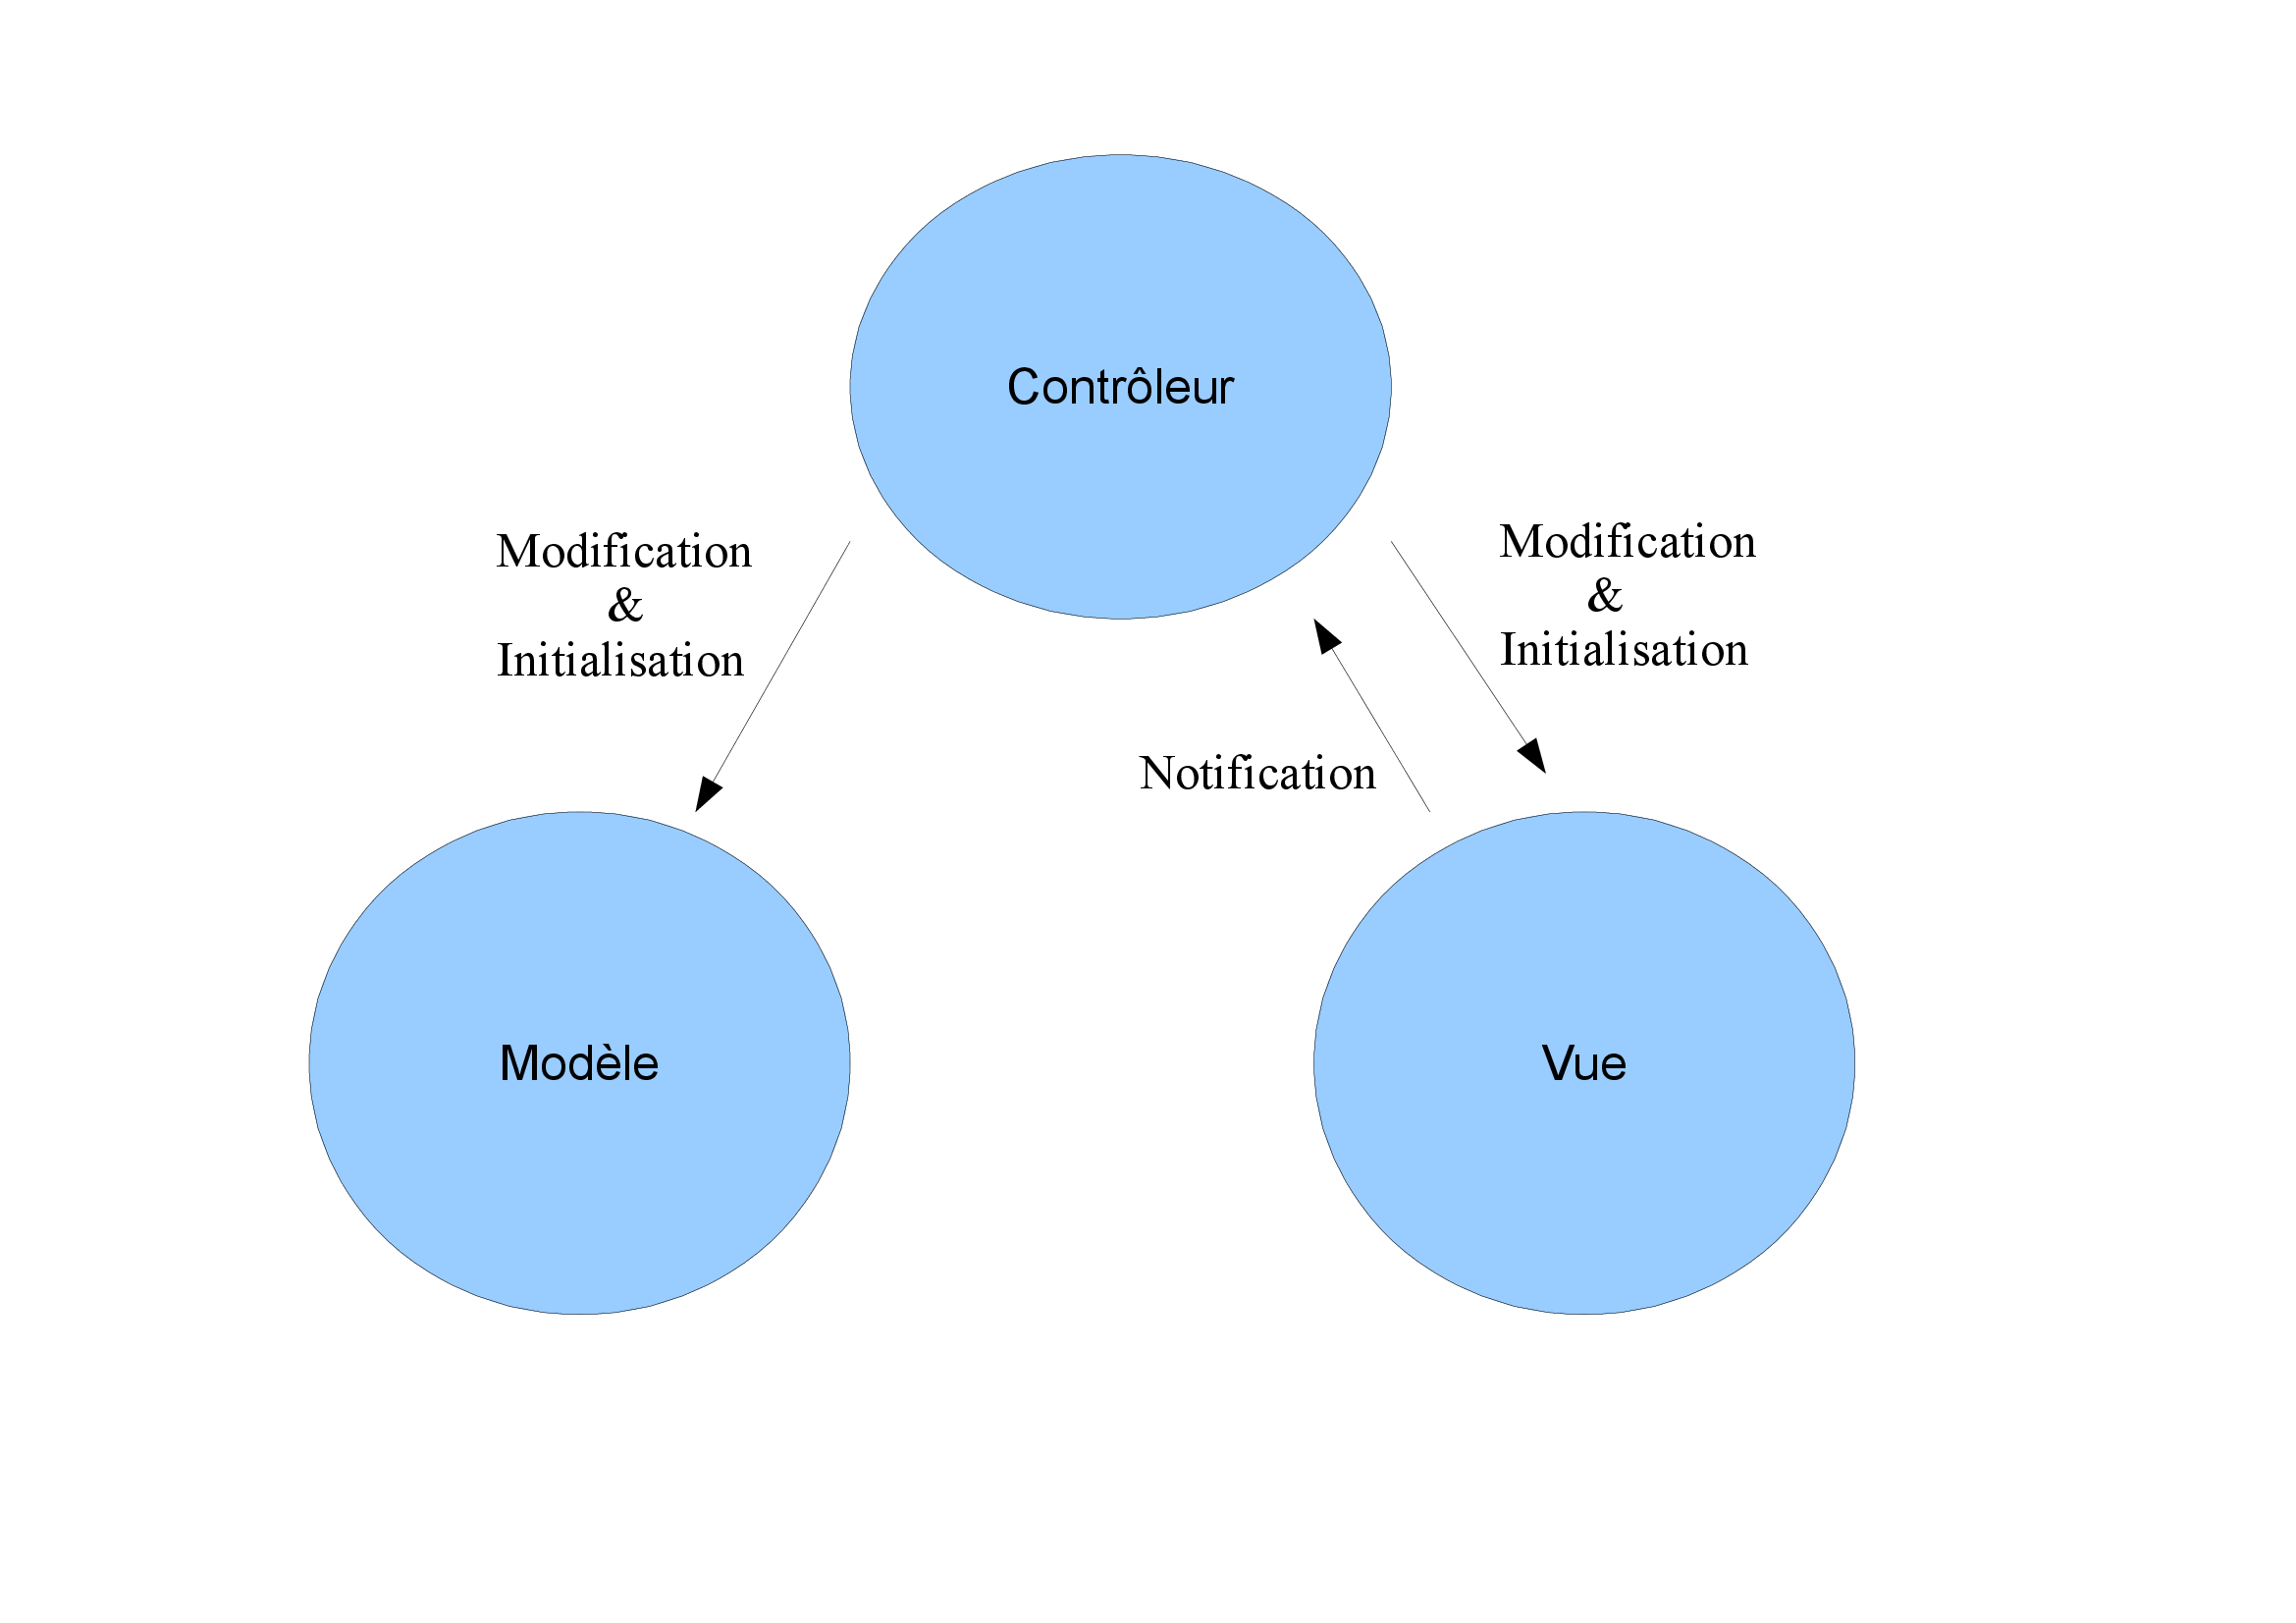
\includegraphics[scale=0.2]{img/mvc.png}

	Nous pouvons remarquer que la classe Controller est une «god class». En effet, tous les traitements effectués passent par cette classe. Lorsqu'on exécute le main, on crée un objet controller qui va générer le modèle et l'interface graphique. En effet, le constructeur de la classe Controller va appeler le constructeur de la classe Game ainsi que celui de la classe RasenderFrame. Ces deux classes correspondent respectivement à notre modèle et à notre vue.
	
	Ensuite, lorsque l'utilisateur va effectuer une action dans l'interface graphique, soit un click de la souris, soit l'appui sur un bouton utilisé dans notre jeu, le contrôleur va être avertit. À partir de là, le modèle va être mis à jour, puis l'interface graphique sera à son tour mise à jour.
	
	 Le fait que cette classe soit une «god class» n'est pas gênant pour ce logiciel. En effet, il n'y a pas de données critiques dans le jeu. Le seul risque est que la partie soit perdu, et que l'utilisateur doive en recommencer une depuis le début.

	
	\subsection{Exemple}
	
	Nous avons vu que le contrôleur initialise et modifie le modèle en fonction des événements que l'interface graphique lui envoie. 
Pour chaque bouton et chaque menu de notre fenêtre nous avons implémenté un «action listener» qui se trouve dans le contrôleur. De plus, pour les événements provenant du clavier ou de la souris, nous avons implémenté les interfaces «MouseListener» et «KeyListener».

	Par exemple, si l'on clique sur le robot rouge dans l'interface graphique, le contrôleur va recevoir cet événement et il va indiquer au modèle le changement à effectuer grâce à la méthode «setSelectedRobot(Robot r)». Ensuite, le contrôleur va avertir l'interface que le modèle a changé en appelant la fonction «refreshBoard». L'interface va donc se mettre à jour et afficher le bon plateau.

\chapter{Explications du code du jeu}
	\section{Fonctionnement du chargement des plateaux}
	
	Le chargement aléatoire du plateau de jeu se fait grâce aux classes Board et BoardPiece. Tout d'abord, la classe Board s'occupe de sélectionner aléatoirement les quatre quarts de plateau avec la face qui sera utilisée. Pour cela, une liste appelée numBoardPieces contenant les quatre entiers 1, 2, 3 et 4 est mélangée et une autre liste de quatre caractères appelée numBoardPiecesSide est remplie aléatoirement avec des A et des B.

	NumBoardPieces correspond aux numéros des quarts de plateau sélectionnés. Le quarts de plateau seront ensuite placés sur le plateau suivant leur position dans la liste :
	\begin{itemize}
	\item[-] 1ère position : en haut à gauche,
	\item[-] 2ème position : en haut à droite,
	\item[-] 3ème position : en bas à droite,
	\item[-] 4ème position : en bas à gauche.
	\end{itemize}

	BoardPiecesSide correspond à la face des quarts de plateau qui sera montrée. La face stockée en première position dans la liste sera appliquée au quart de plateau situé en haut à gauche, celle stockée en deuxième position en haut à droite, etc...
	
	Exemple : 
	\begin{figure}[h!]
	\begin{center}
	  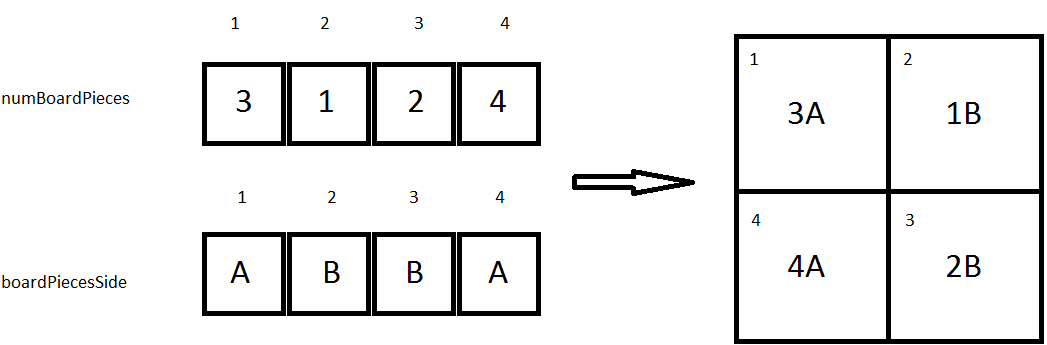
\includegraphics[scale=0.45]{img/SchemaBoard1.png}
	\end{center}
	\end{figure}
	
Ensuite, les quarts de plateau sont initialisés. Quatre BoardPiece sont alors instanciés avec les paramètres suivants:
	\begin{itemize}
	\item[-] Le fichier XML qui contient les informations du quartier,
	\item[-] La position initiale du quartier,
	\item[-] La position finale du quartier.
	\end{itemize}

	Les fichiers XML contiennent toutes les informations des cases spéciales du quart de plateau. C'est-à-dire les cases murées ou qui contiennent une case objectif. Les cases vides, la case grisée centrale ainsi que les murs qui délimitent le plateau ne sont pas enregistrées. Les informations ont été récupérées à partir de photos du plateau de jeu officiel.
	
	\begin{figure}[htbp]
	\begin{minipage}[c]{.45\linewidth}
	\begin{center}
	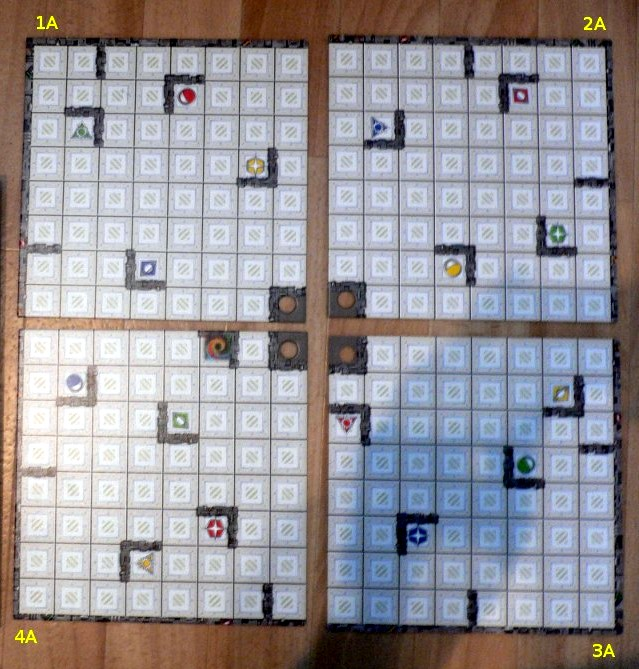
\includegraphics[scale=0.22]{img/img_board_side_A.jpg}
	\label{fig:image1}
	\end{center}
	\end{minipage}
	\hfill
	\begin{minipage}[c]{.45\linewidth}
	\begin{center}
	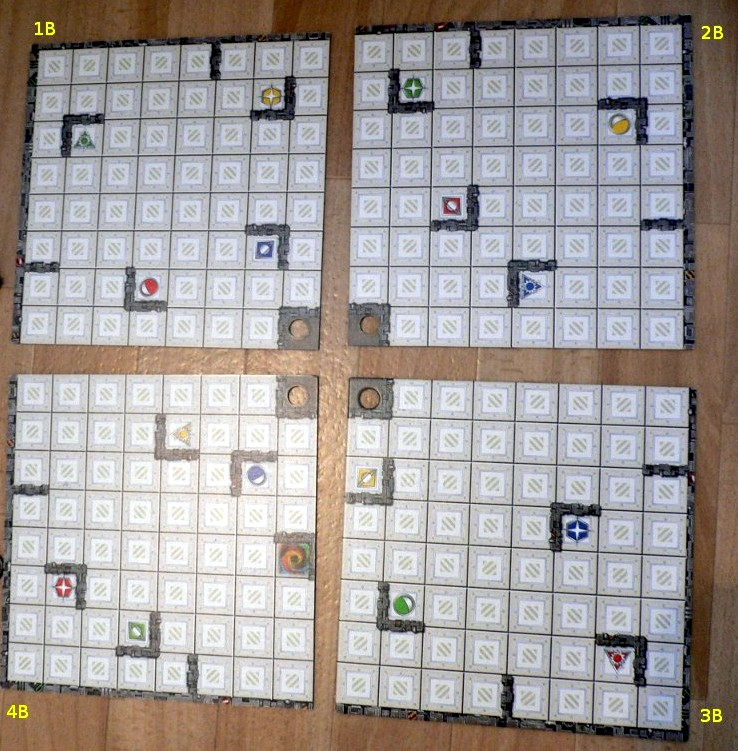
\includegraphics[scale=0.2]{img/img_board_side_B.jpg}
	\label{fig:image2}
	\end{center}
	\end{minipage}
	\caption{Photos des quarts de plateau utilisés.}
	\end{figure}

	
	La position initiale du quartier correspond à la position ou orientation dans laquelle il a été enregistré. Par exemple,le quartier numéro 1 a été enregistré avec sa case centrale positionnée en bas à droite, comme sur la photo.
	
	La position finale est la position que devra occuper le quartier sur le plateau. Ces deux positions servent à calculer quelles sont les rotations nécessaires pour que le quartier soit dans le bon sens. Une fois instanciée, chaque BoardPiece extrait les données des fichiers XML et les stock dans une liste de cases (Box). Les cases contiennent alors leur position sur le quart de plateau, leur type et la position de leurs murs.
	
	Ensuite, les quartiers sont réorientés dans le bon sens avec des rotations. La rotation des cases d'un quartier modifie les positions des cases et l'orientation des murs de chaque case.
	Une soustraction est faite entre la position initiale du quartier et sa position finale pour déterminer les rotations nécessaires :
	\begin{itemize}
	\item[-] différence = 0 : aucune rotation n'est appliquée,
	\item[-] différence = 2 : deux rotations droites sont appliquées,
	\item[-] différence = -1 ou 3 : une rotation droite ou 3 rotations gauches sont nécessaires : la rotation à droite est appliquée,
	\item[-] différence = 1 ou -3 : une rotation gauche ou 3 rotations droites sont nécessaires : la rotation à gauche est appliquée.
	\end{itemize}

	Pour finir, la position des cases sont modifiées par rapport à la position finale du quartier sur le plateau. En effet, le plateau étant plus grand qu'un quartier, la position d'une case sur un quartier n'est pas la même que sur le plateau finale pour les quartiers qui seront placés en 2ème, 3ème et 4ème position sur le plateau :
	\begin{itemize}
	\item[-] position finale = 2 : on décale l'abscisse des cases de 8 vers la droite,
	\item[-] position finale = 3 : on décale l'abscisse des cases de 8 vers la droite et l'ordonnée de 8 vers le bas,
	\item[-] position finale = 4 : on décale l'ordonnée des cases de 8 vers la bas.
	\end{itemize}

	Board peut alors fabriquer le plateau en le remplissant dans une premier temps de cases vides. Board récupère ensuite la liste des cases de chaque BoardPiece et insère les cases dans le plateau. Ensuite, les cases grisées centrales et les murs délimitants le plateau sont placés.
	
	\section{Déplacement des robots}

	L'utilisateur peut déplacer les robots en les sélectionnant à la souris ou au clavier.
	Pour récupérer ces événements, le plateau de jeu doit toujours avoir le focus. Ceci est réalisé grâce à la fonction setFocusOnBoard() appelée dans le contrôleur	quand le plateau perd le focus, c'est-à-dire a quand un bouton de la fenêtre est cliqué. En effet, dès qu'un bouton est cliqué, celui-ci récupère le focus et les évènements du plateau ne sont plus capturés.
	Une fois un évènement clavier ou souris récupéré, le plateau notifie le contrôleur qui traite ces événements en appelant les méthodes correspondantes du modèle.
	Le modèle s'occupe alors de modifier la position du robot sélectionné en le faisant avancer case par case jusqu'à ce qu'il arrive contre un obstacle.

\newpage
\null
\newpage

\chapter{Partie réseau}
	\section{Transmission des données et protocole}
	L'ensemble des classes spécifiques au réseau est regroupé dans le package network. Deux classes séparés permettent de différencier la partie serveur (qui héberge la partie) de la partie client (qui communique uniquement avec serveur).

	Le serveur enregistre la liste des joueurs et donne la main à l'un d'entre eux grâce à la classe PlayerManager. Cette dernière contient un tableau dans lequel les joueurs sont classés dans l'ordre des propositions qu'ils ont réalisé. A chaque fois qu'un joueur passe la main, le compteur de cette classe s'incrémente pour accéder à la case suivante. Le joueur qui a la main en premier est celui qui a fait la plus petite proposition et le plus rapidement (première case du tableau).

	Les données sont formatés à l'aide de la classe protocol qui permet d'encoder et de décoder les différents messages qui sont transmis sous forme de chaîne de caractère (String). Des préfixes au début de chaque message permettent de déterminer quel type de données sont transmises. Les préfixes et données sont séparés au sein d'un même message par un caractère séparateur (typiquement le symbole \&).

	\vspace{0.5cm}
	Exemple :
	\begin{verbatim}
	String robotInfo = ROBOT + "&" + r.x + 
	                           "&" + r.y + 
	                           "&" + r.getColor() + 
	                           "&" + r.originX +
	                           "&" + r.originY;
	\end{verbatim}
    
	\section{Caractéristiques techniques}
	Notre application fonctionne uniquement sur un réseau local avec des adresses du type IPv4. En effet, la plupart du temps sur Internet l'utilisateur se trouve derrière un routeur (une box), il ne nous est pas possible de le gérer à notre niveau. Le port utilisé par le serveur (3001) et différent du port utilisé par le client (3002), cela nous a notamment permis de tester avec une seule machine (en localhost avec l'adresse 127.0.0.1).

	\begin{figure}[h!]
   	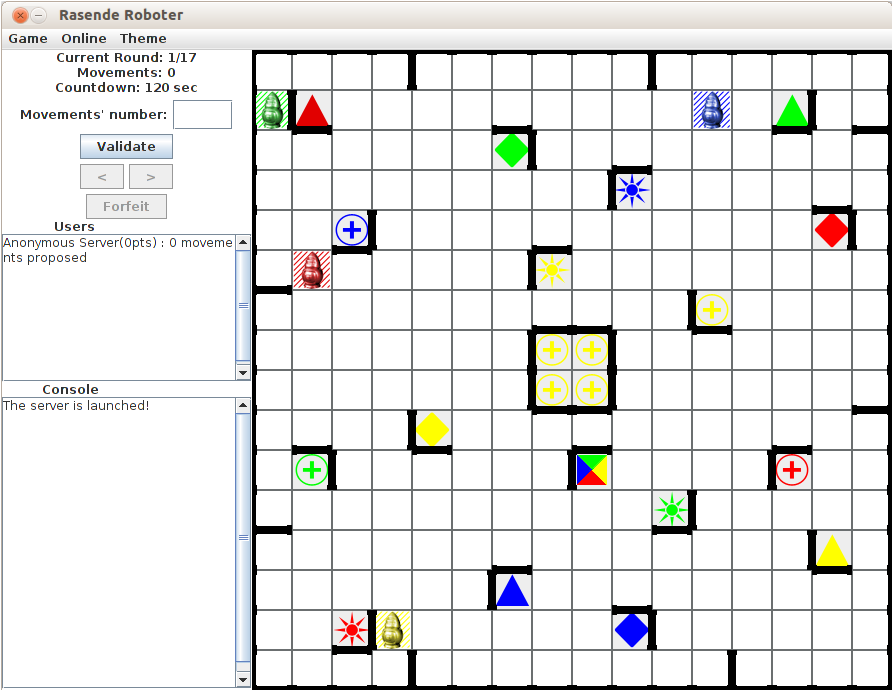
\includegraphics[scale=0.45]{img/multi.png}
	\caption{Vue d'une partie en réseau, avec la colonne de droite qui contient des données supplmentaires par rapport au solo (liste des joueurs, bouton pour déclarer forfait, ...)}
	\end{figure}
	
\newpage
	\section{Glossaire du protocole}
	Liste des préfixes possibles dans le protocole avec les explications sur le type de message transmit à leur suite :
\vspace*{5mm}
	\begin{itemize}
	\item[-] BOARD\_PIECE : envoie l'adresse du quart du fichier xml contenant le plateau à charger et la position où le mettre.
	\item[-] BUTTON\_VALIDATE : permet de dire si le bouton "validate" est actif ou non.
	\item[-] CLIENT : permet d'envoyer la liste des joueurs et leurs données (pseudo, points...) pour l'affichage dans la colonne latérale.
	\item[-] CONNECT : nouvelle connexion entre un client et un serveur.
	\item[-] GOAL\_CARDS : envoie la pile des cases à atteindre.
	\item[-] HAND : permet d'envoyer un message indiquant à un joueur qu'il prend ou perd la main.
	\item[-] MESSAGE : pour transmettre un message à tous, qui s'affichera dans la console latérale du jeu.
	\item[-] MOVE : pour transmettre la position de l'ensemble des robots et le tour courant après un mouvement.
	\item[-] NEXTPROPOSITION : envoyée si un joueur passe la main, permet de demander au serveur de la donner à quelqu'un d'autre
	\item[-] OTHER\_USERNAME : appelé lorsqu'un client essaie de se connecter avec un pseudo déjà pris.
	\item[-] PROPOSITION : permet au client d'envoyer une proposition du nombre de mouvement au serveur.
	\item[-] ROBOT : transmet les données d'un robots au chargement du jeu.
	\item[-] SERVER\_DISCONNECT : permet d'informer les clients que le serveur n'est plus en ligne.
	\item[-] TIME : permet d'envoyer la mise à jour du compte à rebours.
	\end{itemize}

\vspace*{5mm}
	Ce protocole doit être étoffé pour résoudre encore certains problèmes qui apparaissent en réseau, nous n'avons par exemple pas géré le cas d'un client qui se déconnecterait (préfixe possible du message : CLIENT\_DISCONNECT), le server doit dans ce cas le retirer de sa liste et en informer tous les autres clients en mettant à jour leurs listes respectives (en renvoyant un message du type CLIENT).





\newpage
\null
\newpage

\chapter{IA, recherche de solution}

\section{Présentation}
Dans cette partie nous allons vous expliquer en détail comment fonctionne notre IA, et les choix que nous avons faits dans l'implémentation de celle-ci.

\subsection{Structure de données}
Tout d'abord, la structure de données que nous utilisons pour résoudre le jeu se compose de deux tables de hachage et d'une pile. Les tables de hachages nous servent à modéliser un arbre, tandis que la pile a pour fonction d'indiquer à l'utilisateur le chemin à effectuer pour arriver à la solution.

La première table de hachage prend pour \emph{Key} une chaine de caractères qui représente la position de tout les robots à un instant T, et pour \emph{Value} un entier correspondant à la profondeur de la première occurrence de cette configuration. 

La seconde table hachage à comme \emph{Key} la même chaine de caractères, mais comme \emph{Value} la position des robots "père".

La pile contient l'ensemble des clés qui composent le chemin solution.

\subsection{Système de clé}
Comme dit plus haut, la \emph{Key} des tables de hachage est une chaine de caractères spéciale contenant la position des robots à un instant donné.

La chaine de caractères est de la forme : 

\emph{PositionXRobotBleu;PositionYRobotBleu;Bleu\&PositionXRobotVert;…}

\subsection{Avantages}
Nous avons choisi d'implémenter notre IA en utilisant des tables de hachage car elles permettent de s'assurer de l'unicité des \emph{Keys}. C'est un point très important car si une configuration de robots apparait alors qu'elle est déjà dans la table de hachage cela signifie qu'elle a déjà été traitée et que donc il n'est pas nécessaire de la retraiter. Cela permet de réduire grandement le nombre de cas à traiter à chaque profondeur.

De plus, nous avons choisi d'utiliser une chaine de caractères comme \emph{Key} pour les tables de hachage plutôt que la liste de tous les robots car il est plus facile et plus efficace de comparer deux chaines de caractères plutôt que deux listes d'objets.

\section{Recherche de la solution}

\subsection{Initialisation}
Lors de l'initialisation de notre algorithme, la position courante des robots est transmise à notre algorithme. Il crée alors la clé racine qu'il ajoute dans la première table de hachage à la profondeur 0.

\subsection{Itération}
Par la suite, tant que la solution n'a pas été trouvée nous répétons les étapes suivantes :

\begin{itemize}
\item Nous récupérons l'ensemble des \emph{Keys} qui ont pour \emph{Value} depth-1 (c'est-à-dire toutes les clés ajoutées lors de la précédente itération)

\item Chaque clé est ensuite décomposée de façon à obtenir la configuration des robots associée.

\item Chaque robot est déplacé dans toutes les directions dans lesquelles il peut bouger. C'est-à-dire dans toutes les directions où il n'est pas obstrué par un mur ou un autre robot.

\item Pour chaque déplacement du robot nous reconstruisons la clé associée à cette nouvelle configuration du plateau.

\item Si ce déplacement est un déplacement gagnant, la clé est conservée comme étant la feuille de l'arbre et sera utilisée pour la reconstruction du chemin parcouru.

\item Sinon, on ajoute cette clé dans la table de hachage en s'assurant qu'elle n'y soit pas déjà. Si elle n'y est pas, on l'ajoute également dans la seconde table de hachage servant à reconstruire la solution, avec comme \emph{Value} la clé père.
\end{itemize}

\subsection{Reconstruction du chemin}
Une fois la solution trouvée, nous remontons de père en fils grâce à la seconde table de hachage, et nous stockons à chaque itération la clé fils dans la première pile. 

Ensuite, nous comparons deux a deux les clés contenues dans pile, pour pouvoir retrouver la direction dans laquelle s'est déplacé le robot entre sa première et sa seconde position. Cette opération à pour but d'indiquer à l'utilisateur la direction dans laquelle doit déplacer le robot.

\section{Amélioration possible}
La version actuelle de notre algorithme nous permet de traiter un maximum d'environ un million de possibilités différentes, ce qui permet de trouver des solutions en environ 15 coups maximum.

Une amélioration possible serait de créer un algorithme qui attribuerait un poids aux possibilités de la profondeur d'arrêt. Cette pondération serait utilisée pour déterminer quelle possibilité peut être utilisée pour relancer l'algorithme.


\newpage
\null
\newpage

\chapter{Tests}
Quatre types de tests ont été effectués : tests unitaires pour vérifier une fonction ou une partie du code, des tests de test de non régression, des Stress Test afin de connaitre quelques limites de notre programme et aussi des tests manuels sur l'interface graphique (boutons, menus...).

Les JUnit tests (contenus dans le package test) peuvent tous être lancés à la suite grâce à la classe AllTests. Les outils de taux de couverture nous donnent un chiffre de 60,5 %.

\section{JUnit tests}
\begin{itemize}
	\item BoxTest : ce fichier teste si une fois que la case est créée les murs sont au bon endroit et dans quelles directions peut ou non aller un robot qui la traverse.
	\item ClientTest : un client est créé. On teste l'encodage et le décodage d'un message qui transmet la position des robots et celui qui transmet une nouvelle main.
	\item Controllertest : teste le déplacement des robots dans une direction choisie.
	\item CountDownTest : permet de vérifier que le compte à rebours fonctionne (initialisation, arrêt, reset, démarrage).
	\item GameTest : Test les différents éléments à la création d'une nouvelle partie ainsi que les fonctions de sélection des robots.
	\item NetworkTest : vérifications à la création d'un client et un serveur.
	\item PlayerManagerTest : permet de tester le tableau qui gère la liste des joueurs d'un serveur en fonction des propositions effectuées, des suppressions de joueurs ou des changements de propositions de mouvements.
	\item PlayerTest : permet de tester les données liées aux joueurs.
	\item ProtocolTest : teste l'encodage et le décodage de messages. Vérifie que les données récupérées après le décodage soient les mêmes qu'avant l'envoi.
	\item RobotTest : vérifie la position des robots après qu'ils soient placés sur un plateau
	\item StructTreeTest : essais d'ajout d'éléments dans notre arbre de la solution du chemin.
\end{itemize}

\section{Stress Tests}
Ils ont été réalisés afin de déterminer la robustesse du jeu dans certaines situations.
On a donc pu ainsi déterminer que notre algorithme de résolution avait une limite à 15 dans l'arbre des solutions. C'est ce qui nous a permis d'arrêter notre recherche pour demander à l'utilisateur d'effectuer d'autres mouvements avant de la relancer.

Le réseau a aussi pu être testé avec cinq machines d'un réseau local sans problèmes. Cela correspond à un joueur qui héberge le serveur et quatre clients. N'ayant pas eu l'occasion de tester à plus grande échelle, nous avons choisi de ne pas mettre de limite au nombre de connexions simultanés.


\section{Tests manuels}
Tous les élements graphiques ont étés testés :
	\begin{itemize}
	\item Les boutons.
	\item Les menus.
	\item Les zones de texte qui attendent des valeurs (il n'est donc pas possible de rentrer une adresse IP avec un format incorect ou de proposer un nombre de mouvement négatif).
	\end{itemize}
Le jeu a également été testé sur Linux et MAC comme demendé par les clients mais aussi sur Windows.


\begin{comment}
\section{Tests mise en place et génération de la carte}
\begin{itemize}
	\item[-] Vérifier qu'une carte contient les 17 cases objectif.
	\item[-] Vérifier qu'il n'existe pas de cases objectifs identiques (couple couleur/forme)
	\item[-] Vérifier que chacun des robots est sur la case de départ correspondant à sa couleur.
	\item[-] Vérifier qu'une case objectif possède deux murs concomitants (pour permettre à un robot de s'y arrêter et de repartir dans une autre direction).
	\item[-] Vérifier qu'il n'existe pas de zones fermées (hormis la zone centrale).
	\item[-] Les compteurs de points des joueurs, du nombre de tours et de déplacements doivent tous être initialisés à 0.
\end{itemize}

\section{Tests déplacements des robots}
\begin{itemize}
	\item[-] Tester les déplacements dans les quatre directions possibles.
	\item[-] Tester des déplacements avec un arrêt devant un mur, un arrêt devant un autre robot et un arrêt au bord de la carte : vérifier à chaque fois que la position du robot est bien avant l'obstacle.
	\item[-] Tester l'arrêt sur une case objectif et vérifier que le compteur de point du joueur s'incrémente (avec un pas de 1).
\end{itemize}

\section{Tests sur l'interface graphique}
\begin{itemize}
	\item[-] Il faut tester chaque passage d'une fenêtre à une autre (via les boutons) et dans les deux sens. Exemple : du menu vers la partie solo et inversement.
	\item[-] Vérifier que les images ont des noms valides.
	\item[-] Vérifier que la couleur et le motif d'une case correspond bien à celui de l'image.
\end{itemize}

\section{Tests sur la partie réseau}
\begin{itemize}
	\item[-] Tester les adresses IP avec format correct et incorrect.
	\item[-] Calculer le nombre limite de connections simultanées sur un serveur.
	\item[-] Test sur la synchronisation des joueurs.
	\item[-] Tester ce qui se passe en cas d’arrêt du serveur en cours de partie.
	\item[-] Tester ce qui se passe si un joueur quitte une partie en cours.
\end{itemize}

\section{Tests sur l'algorithme (IA)}
\begin{itemize}
	\item[-] Tester sans se préoccuper des autres robots et inversement.
	\item[-] Mesurer le temps d'exécution moyen.
\end{itemize}

\section{Tests sur le déroulement d'une partie}
\begin{itemize}
	\item[-] Vérifier qu'une partie en réseau ne peut commencer qu'avec deux joueurs minimum.
	\item[-] Vérifier que la fin du chrono déclenche bien une des deux actions associées : soit le passage à un autre joueur qui a donné une solution avec plus de coup soit un point de plus pour le joueur qui vient de trouver le plus petit nombre de déplacements.
		\item[-] La somme des points des joueurs ne peut jamais dépasser le nombre de case objectifs. S'il y a égalité, cela signifie que tous les objectifs ont été atteints, donc que la partie est terminée.
\end{itemize}	

\end{comment}


\chapter*{Conclusion}
\addcontentsline{toc}{chapter}{Conclusion}

	Globalement, les trois principales priorités ont été réalisées, le solo est entièrement fonctionnel et permet au joueur de faire les 17 niveaux du jeu à son rythme. Dans le cas où il ne trouve pas la solution par lui-même, il peut faire intervenir le solver qui va lui donner les mouvements à effectuer via la console latérale. Cette solution est optimale dans le sens où il s'agit de l'un des meilleurs chemins possibles pour le robot. Une solution est trouvée pour tous les cas inférieurs ou égaux à 15 mouvements. Au-delà, on ne peut pas encore trouver de solution. Des possibilités d'améliorations via une heuristique qui relancerait notre algorithme sont possibles. 

	Le jeu fonctionne aussi en réseau local, cependant des problèmes de gestion en cas de déconnexion de clients par exemple n'ont pas été gérés. Même si d'autres cas ont été traités (par exemple déconnexion du serveur), il reste encore cette partie sécurité à améliorer.

	Afin d'améliorer l'esprit jeu de ce Ricochet Robots, il pourrait être intéressant de permettre à l'utilisateur une plus grande personnalisation. C'est déjà le cas avec la possibilité d'un thème différant mais d'autres options peuvent être envisagées : autres couleurs pour les robots, plus ou moins de symbole, cartes supplémentaires...



\appendix
\chapter*{Annexes}
\addcontentsline{toc}{chapter}{Annexes}


\nocite*
\bibliographystyle{plain}
\bibliography{biblio}
\end{document}
